\section{Malla Desplazada (Staggered Grid)}

\subsection{Condiciones de contorno}
Se utilizan nodos ficticios para establecer las condiciones de frontera tipo Dirichlet o Neumann. Se utiliza la Figura \ref{fig1} como referencia.

\paragraph{Condiciones de Dirichlet} Utilizando una malla desplaza se observa que para ciertos bordes las condiciones se pueden implementar naturalemente. Sin embargo las condiciones de no deslizamiento en la pared superior no se pueden imponer directamente para $u$ (de la misma manera, en el lado izquierdo del borde no se pueden imponer directamente la condición de $v=0$) Para lograr ello se emplean nodos ficticios que sobresalen los contornos del dominio. Utilizando esquemas CDS se puede imponer que la velocidad $u$ en $\partial \Omega$ sea nulo

\begin{equation}
\dfrac{1}{2} (u + u_f) = 0 \rightarrow u_f = -u
\end{equation}

análogo para la componente vertical

\begin{equation}
\dfrac{1}{2} (v + v_f) = 0 \rightarrow v_f = -v
\end{equation}

El ejemplo se extiende a cualquier valor de velocidad $\vec{v} = \left\{ \overline{u}, \overline{v} \right\}$ en el contorno

\paragraph{Condiciones de Neumann} Se utiliza la misma lógica para imponer las condiciones de flujo en los contornos. Por ejemplo, para la variable $u$ se fija una condiciones de flujo nulo en los contornos y empleando un esquema CDS en el lado izquierdo se tiene:

\begin{equation}
\dfrac{\partial \hat{u}}{\partial x} \Big|_{\Gamma_u} \approx \dfrac{\hat{u}-\hat{u}_f}{\Delta x} = 0  \rightarrow  \hat{u}_f = \hat{u}
\end{equation}

\begin{figure} [H]
\centering
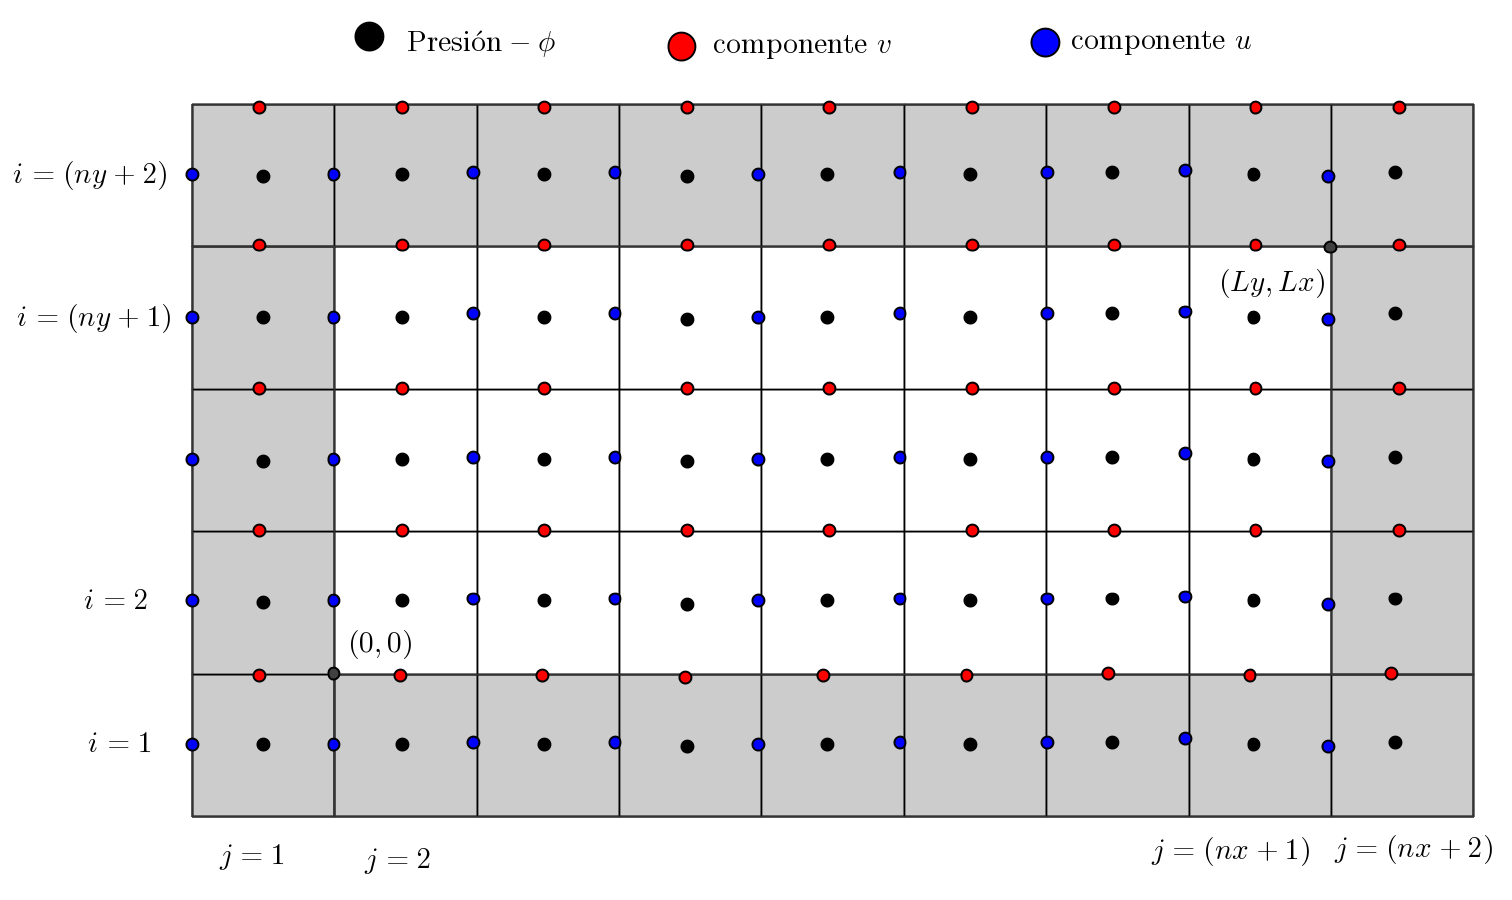
\includegraphics[width=0.8\textwidth]{malla.png}
\caption{Esquema representativo. Círculos azules: $u$ ; Rectángulos rojos: $v$ ; Equis : $P$} \label{fig1}
\end{figure}